\documentclass{beamer}
\usepackage[utf8]{inputenc}

\usetheme{Madrid}
\usecolortheme{default}
\usepackage{amsmath,amssymb,amsfonts,amsthm}
\usepackage{txfonts}
\usepackage{tkz-euclide}
\usepackage{listings}
\usepackage{adjustbox}
\usepackage{array}
\usepackage{tabularx}
\usepackage{gvv}
\usepackage{lmodern}
\usepackage{circuitikz}
\usepackage{tikz}
\usepackage{graphicx}

\setbeamertemplate{page number in head/foot}[totalframenumber]

\usepackage{tcolorbox}
\tcbuselibrary{minted,breakable,xparse,skins}



\definecolor{bg}{gray}{0.95}
\DeclareTCBListing{mintedbox}{O{}m!O{}}{%
	breakable=true,
	listing engine=minted,
	listing only,
	minted language=#2,
	minted style=default,
	minted options={%
		linenos,
		gobble=0,
		breaklines=true,
		breakafter=,,
		fontsize=\small,
		numbersep=8pt,
		#1},
	boxsep=0pt,
	left skip=0pt,
	right skip=0pt,
	left=25pt,
	right=0pt,
	top=3pt,
	bottom=3pt,
	arc=5pt,
	leftrule=0pt,
	rightrule=0pt,
	bottomrule=2pt,
	toprule=2pt,
	colback=bg,
	colframe=orange!70,
	enhanced,
	overlay={%
		\begin{tcbclipinterior}
			\fill[orange!20!white] (frame.south west) rectangle ([xshift=20pt]frame.north west);
	\end{tcbclipinterior}},
	#3,
}
\lstset{
	language=C,
	basicstyle=\ttfamily\small,
	keywordstyle=\color{blue},
	stringstyle=\color{orange},
	commentstyle=\color{green!60!black},
	numbers=left,
	numberstyle=\tiny\color{gray},
	breaklines=true,
	showstringspaces=false,
}
%------------------------------------------------------------
%This block of code defines the information to appear in the
%Title page
\title %optional
{1.5.34}
%\subtitle{A short story}

\author % (optional)
{RAVULA SHASHANK REDDY - EE25BTECH11047}



 \begin{document}
	
	
	\frame{\titlepage}
	\begin{frame}{Question}
		The point P which divides the line segment joining the points A (2, -5)
		and B (5,2) in the ratio 2 : 3 lies in which quadrant?
	\end{frame}
	\begin{frame}{allowframebreaks}
		\frametitle{Equation}
	\textbf{The formula for internal division of vectors is where $\vec{P}$ divides $\vec{A}$ and $\vec{B}$ in the ratio k:1}
		\centering
		
		\label{tab:parameters}
		\begin{align*}
			\vec{P} =	\frac{k\vec{B} + \vec{A}}{1+k} 
		\end{align*}
		\end{frame}	
	
	\begin{frame}{Theoretical Solution}
    Given:
\begin{align}
\vec{A} = \myvec{2 \\ -5} \\ \vec{B} = \myvec{5 \\ 2}
\end{align}

Now the matrix form for $\vec{A}$ and $\vec{B}$ is :
\begin{align}
    \myvec{\vec{A} & \vec{B}} = \myvec{2 & 5 \\ -5 & 2}
\end{align}
The point \(P\) dividing the segment \(AB\) in the ratio 2:3 internally , has the position vector :
\begin{align}
\vec{P} = \frac{ 3\vec{A} +2\vec{B} }{3+2} 
\end{align}
\end{frame}
\begin{frame}
Thus by using the section formula \\
\begin{align} 
\vec{P}= \frac{1}{5} \cdot \myvec{\vec{A} & \vec{B}}\myvec{3 \\ 2}\\
\vec{P}= \frac{1}{5} \cdot \myvec{2 & 5 \\ -5 & 2}\myvec{3 \\ 2}\\
\vec{P}= \frac{1}{5} \cdot \myvec{6 + 10\\ -15 + 4}\\
\therefore \vec{P}= \frac{\myvec{16 \\ -11}}{5}.
\end{align}

Hence the vector $\vec{P}$ is \myvec{\frac{16}{5} \\ \frac{-11}{5}}  = \myvec{3.2 \\ -2.2} \\
Since \(x>0\) and \(y<0\), $\vec{P}$ lies in the \textbf{IV (fourth) quadrant}.

\end{frame}
	
	\begin{frame}[fragile]
		\frametitle{C Code - Section formula function }
		
		\begin{lstlisting}
// section_formula.c
#include <stdio.h>

void find_section_point(double x1, double y1, double x2, double y2, double m, double n, double* x, double* y) {
	*x = (m * x2 + n * x1) / (m + n);
	*y = (m * y2 + n * y1) / (m + n);
}
			\end{lstlisting}
		\end{frame}


\begin{frame}[fragile]
	\frametitle{Python Code through shared output}
	\begin{lstlisting}
# Section Formula Problem

import numpy as np
import matplotlib.pyplot as plt

# Given points
A = np.array(([2, -5])).reshape(-1,1)
B = np.array(([5, 2])).reshape(-1,1)

# Ratio m:n = 2:3
m, n = 2, 3

# Point dividing AB in ratio m:n
P = (n*A + m*B) / (m+n)

# Determine Quadrant
x, y = P[0,0], P[1,0]
	\end{lstlisting}
\end{frame}

\begin{frame}[fragile]
	\begin{lstlisting}
if x > 0 and y > 0:
    quadrant = "First Quadrant"
elif x < 0 and y > 0:
    quadrant = "Second Quadrant"
elif x < 0 and y < 0:
    quadrant = "Third Quadrant"
elif x > 0 and y < 0:
    quadrant = "Fourth Quadrant"
else:
    quadrant = "On Axis"

print(f"Coordinates of P: ({x:.2f}, {y:.2f})")
print(f"P lies in the {quadrant}")

# Generate line AB
x_AB = np.linspace(A[0,0], B[0,0], 100)
y_AB = np.linspace(A[1,0], B[1,0], 100)

	\end{lstlisting}
\end{frame}

\begin{frame}[fragile]
	
	\begin{lstlisting}
# Plot line AB
plt.plot(x_AB, y_AB, label='$AB$')

# Plot points A, B, P
plt.scatter([A[0,0], B[0,0], P[0,0]], [A[1,0], B[1,0], P[1,0]], color='red')
labels = ['A(2,-5)', 'B(5,2)', f'P({x:.2f},{y:.2f})']
for i, txt in enumerate(labels):
    plt.annotate(txt, ( [A[0,0], B[0,0], P[0,0]][i],
                        [A[1,0], B[1,0], P[1,0]][i]),
                 textcoords="offset points", xytext=(10,-10))
	\end{lstlisting}
\end{frame}
\begin{frame}[fragile]
	
	\begin{lstlisting}
# Styling axes
ax = plt.gca()
ax.spines['left'].set_position('zero')
ax.spines['bottom'].set_position('zero')
ax.spines['top'].set_color('none')
ax.spines['right'].set_color('none')

plt.legend(loc='best')
plt.grid(True)
plt.axis('equal')
plt.show()

	\end{lstlisting}
\end{frame}

	\begin{frame}[fragile]
\frametitle{Python code : Direct }

\begin{lstlisting}
import numpy as np
import matplotlib.pyplot as plt
#local imports
from libs.line.funcs import *
from libs.triangle.funcs import *
from libs.conics.funcs import circ_gen


# Given points
A = np.array(([2,-5])).reshape(-1,1)
B = np.array(([5,2])).reshape(-1,1)

# Ratio m:n = 2:3
m, n = 2, 3

# Point dividing AB in ratio m:n
P = (n*A + m*B) / (m+n)
\end{lstlisting}
\end{frame}

\begin{frame}[fragile]

\begin{lstlisting}
# Generating line AB
def line_gen(A,B):

    len = 100
    dim = A.shape[0]
    x_AB = np.zeros((dim,len))
    lam_1 = np.linspace(0,1,len)
    
    
    for i in range(len):
        temp1 = A + lam_1[i]*(B-A)
        x_AB[:,i]= temp1.T
    return x_AB

x_AB = line_gen(A,B)

# Plotting line AB
plt.plot(x_AB[0,:], x_AB[1,:], label='$AB$')

# Plotting points A, B, P
\end{lstlisting}
\end{frame}

\begin{frame}[fragile]

\begin{lstlisting}
tri_coords = np.block([[A,B,P]])
plt.scatter(tri_coords[0,:], tri_coords[1,:])
vert_labels = ['A','B','P']

for i, txt in enumerate(vert_labels):
    plt.annotate(f'{txt}\n({tri_coords[0,i]:.1f}, {tri_coords[1,i]:.1f})',
                 (tri_coords[0,i], tri_coords[1,i]),
                 textcoords="offset points",
                 xytext=(20,-10), ha='center')

# Axis styling
ax = plt.gca()
ax.spines['left'].set_position('zero')
ax.spines['bottom'].set_position('zero')
ax.spines['top'].set_color('none')
ax.spines['right'].set_color('none')
\end{lstlisting}
\end{frame}

\begin{frame}[fragile]

\begin{lstlisting}
plt.legend(loc='best')
plt.grid()
plt.axis('equal')
plt.show()
\end{lstlisting}
\end{frame}


\begin{frame}{Plot by python using shared output from c}
	\begin{center}
		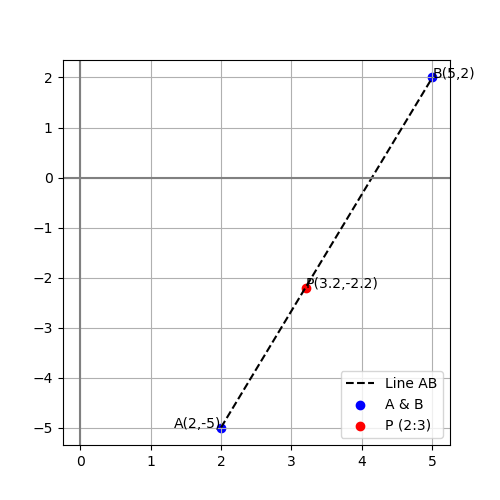
\includegraphics[width=0.6\columnwidth]{figs/fig_1.png}
	\end{center}
\end{frame}

\begin{frame}{Plot by python only}
	\begin{center}
		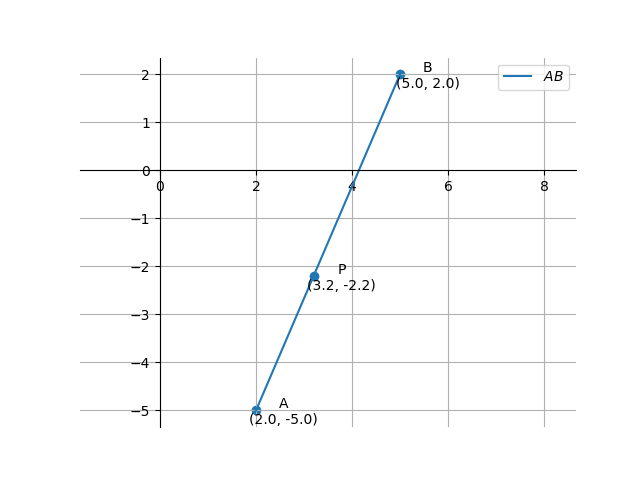
\includegraphics[width=0.8\columnwidth]{figs/fig_2.png}
	\end{center}
\end{frame}



\end{document}